\chapter{Surface-tension driven open microfluidic platform for hanging droplet culture}\footnote{This chapter has been modified from the published manuscript of the same title. The manuscript includes as authors Theodorus de Groot, Kelsey Veserat, Erwin Berthier, Ashleigh Theberge, and David Beebe}
\label{Chap:HangingDroplet}

The hanging droplet technique for three-dimensional tissue culture has been used for decades in biology labs, with the core technology remaining relatively unchanged. Recently microscale approaches have expanded the capabilities of the hanging droplet method, making it more user-friendly. We present a spontaneously driven, open hanging droplet culture platform to address many limitations of current platforms. Our platform makes use of two interconnected hanging droplet wells, a larger well where cells are cultured and a smaller well for user interface \textit{via} a pipette. The two-well system results in lower shear stress in the culture well during fluid exchange, enabling shear sensitive or non-adherent cells to be cultured in a droplet. The ability to perform fluid exchanges in-droplet enables long-term culture, treatment, and characterization without disruption of the culture. The open well format of the platform was utilized to perform time-dependent coculture, enabling culture configurations with bone tissue scaffolds and cells grown in suspension. The open nature of the system allowed the direct addition or removal of tissue over the course of an experiment, manipulations that would be impractical in other microfluidic or hanging droplet culture platforms. 


\section{Introduction}
Hanging droplet culture is perhaps the earliest 3D tissue culture system developed \cite{Harrison1910}. This method relies on the 3D self-assembly of a tissue spheroid from a cell suspension within a droplet suspended from the lid of a Petri dish. The earliest hanging droplet culture platform enabled the in vitro study of embryo development \cite{Harrison1910}, but the technique would later be used to study stem cell differentiation, tumorigenesis, bacteria \cite{Tittsler1936}, and even plant culture \cite{Muir1958}. In mammalian tissue culture, 3D techniques are capable of better replicating the in vivo environment, and observations made in 3D systems are often more physiologically relevant than in 2D cultures \cite{Abbott2003, Stegemann2003, Debnath2005, Folkman1973}. Despite the biological advances enabled by hanging droplet culture, the method has several limitations, including inconsistencies in droplet size and challenges accessing the culture for fluid exchange. To address the limitations of the traditional hanging drop technique, new methods of spheroid culture have been developed as a means to rapidly and consistently create 3D cultures including low-adhesion culture surfaces \cite{Turner2014}, natural or synthetic extracellular matrix gels \cite{Debnath2005, Karthaus2014, Lee2012} and microfluidic approaches \cite{Hsiao2009, Wu2008}. The hanging droplet technique has been transformed recently through the use of an open well design, thereby allowing pipette and liquid handling robot access to the wells and enabling high-throughput screening of 3D tissue cultures \cite{Tung2011}. Microfluidic techniques have since been used to improve on the capabilities of the hanging drop approach. Frey \textit{et al.}  developed hanging droplet wells connected through microchannels, which were used to create directional transfer of media between separate organoids each in their own droplet in a body-on-a-chip approach \cite{Frey2014}. Importantly, they observed that connected hanging drops would spontaneously equilibrate volume based on the surface tension at the air-liquid interface.

Traditional microfluidic platforms utilize closed channels, enclosed on all sides with the exception of wells used to move fluid into and out of the device. In contrast, open microfluidic devices have at least one area of the device open to air \cite{Kaigala2012, Zimmermann2005a, Walker2002}. These platforms leverage the innate physical properties of water at small volumes to drive critical microfluidic operations such as fluid exchange. Devices with fluid constrained between only two faces have emerged as well. These completely open microfluidic platforms, or 'suspended microfluidics', offer advantages for tissue culture by providing access to interface directly with not only the media but also cells and organoids in the culture without obstruction from closed channels. This eliminates the need for tubing and pumps and allows interfacing with a pipette tip or liquid handling robot for bench work or high-throughput applications and enables fluid flow entirely through surface tension-driven capillary action A variety of applications and functions have been realized in open platforms. For example, a suspended microfluidics platform enabled screening assays, three-dimensional (3D) cell invasion assays, microscale metabolomics, and micromembrane formation \cite{Casavant2013}. While open microfluidics currently drives a very small portion of microculture devices, it has great potential to improve current platforms and enable new and unique culture configurations. We endeavored to bring the advantages of open microfluidics to the widely used hanging droplet culture method.

Here, we build upon the innovations of recent open microfluidics and hanging droplet culture approaches to develop a versatile hanging drop platform, capable of increased biological complexity while maintaining the same ease-of-use as contemporary hanging droplet platforms. The platform consists of two connected and open droplets, a culture droplet and a user interface droplet. The open design of each droplet allows for cells or tissues to be added to and removed from culture dynamically over the course of an experiment. The connected droplet approach serves to dampen fluid exchange through a surface tension driven phenomenon similar to passive pumping previously described by Walker \textit{et al.}  \cite{Beebe2002a}.  Specifically, pressure in a smaller droplet is higher than pressure in a larger droplet due to surface tension effects; we utilize pressure differences between connected droplets of differing diameters to shuttle fluids from one droplet to the other.  We perform a full characterization of the forces that control fluid flow in our system and validate the model empirically. The interface droplet enables long-term culture in the hanging drop and the application of treatments to the culture with minimal disturbance to the cells in the droplet making the platform well-suited for shear-sensitive cell types, such as suspension cells which are considerably more difficult to culture in microdevices compared to adherent cell types \cite{Young2012}. 

\section{Methods}
\subsection{Device Fabrication}
Devices were designed and modeled with 3D modeling software (Solidworks, Dessault Systems, France). Devices were CNC milled (Tormach, Waunakee, WI) from clear 1.2 mm polystyrene sheets (Goodfellow, Coraopolis, PA) as described by Guckenberger \textit{et al.}  \cite{Guckenberger2015} After milling, each device was rinsed with DI water and sonicated for 5 minutes in 100\% isopropyl alcohol to remove any residual coolant or chips from the milling process and stored in lint-free wipes. All double-well hanging droplet devices used had a smaller well diameter of 4 mm and a larger well diameter of 4.25 mm with a connecting channel 0.75 mm long with a width and height of 0.6 mm (3D model files attached in ESI).

\subsection{Computational Modeling}
A numerical model to describe the double hanging drop system was developed using MATLAB (Mathworks, Natick, MA). We implemented a two-tiered iterative numerical modeling approach. In the first tier, we solve the equilibrium state for each drop given a certain overall volume. Based on the work developed by Carvajal \textit{et al.}  \cite{Carvajal2011} that describes the shape, volume, and pressure in the pendant drop given the height of its apex, we calculated a reference table to back-calculate the hanging drop characteristics as a function of the volume of the drop. Using this function, we iteratively equilibrated the top and bottom air-liquid interface of a hanging drop by exchanging small volumes of liquid between the higher pressure interface and the lower pressure interface until both pressures matched within 10-3 Pa. Once each individual hanging drop was equilibrated, a small volume of liquid, proportional to the difference in pressure between the two hanging drops and the inversely proportional to the fluidic resistance of the joining channel, is exchanged between the two hanging drops. The process is then repeated to equilibrate the adjoining hanging drops until the pressure difference between the two hanging drops is less than 10-3 Pa. The model was validated experimentally with a device with the same dimensions, and volumes were compared by imaging the device with a goniometer (ram\'{e}-heart, inc. Mountain Lakes, NJ) and calculating the volume in each well.

\subsection{Suspension cell culture}
Prior to culture, cleaned devices were placed onto 3D-printed PLA inserts (Makerbot Industries, Brooklyn, NY), then into OmniTrays (Thermo Scientific, Waltham, MA). The devices were sterilized through exposure to UV light for at least 30 minutes. Wells on the device inserts as well as the bottom of the OmniTray were filled with water to provide humidity to the wells and prevent fluid evaporation in a similar setup validated by Tung et. al \cite{Tung2011} (Fig. \ref{figure:FigS1}). Evaporation was further mediated by placing the device in the rear of the humidified tissue culture incubator to avoid temperature gradients \cite{Berthier2008}. Devices were filled with a total of 60 \textmu L of fresh media. 20,000 MM.1S cells were seeded into the culture well of each device in a bolus of 2 \textmu L of media. Cells were left for at least 24 h in wells to settle prior to experimentation.  

\subsection{One- and two-well comparison}
In addition to the two hanging drop devices, we fabricated single-well devices with a diameter of 4.25 mm in order to directly compare the functionality of one- and two- well devices. Two-well devices were prepared as previously mentioned, however, single-well devices were filled with 35 \textmu L of media, the same volume as measured in the larger well of the two-well system. Both single- and two-well devices were seeded following the protocol described in section 2.3. 

For Fig. 3A, pipetting was performed using a multi-channel liquid handling robot (PipeteMax, Gilson, Madison, WI). Pipetting in the two-well device was done at the interface well, while pipetting was performed in the culture well of the one-well device. Wells were subjected to either 0, 1, 3, or 5 pipetting steps, which involved aspiration and redispensing of 20 \textmu L and 12 \textmu L for the two- and single- well devices, respectively, at a flow rate of 1 mL /min. Immediately following pipetting, brightfield images at 4x magnification were acquired (IX-81, Olympus, Tokyo, JP).
Particle image velocimetry (PIV) was used to compare velocities in single- and double-well device systems during pipetting. Devices were placed on a fluorescence microscope and filled with 15 m blue fluorescent beads diluted in 1XPBS. The microscope was focused on the bottom of the droplet and more beads diluted in 1XPBS were added using an electronic pipette replicating the liquid handling robot. The images acquired were analyzed with the PIV ImageJ (http://rsb.info.nih.gov/ij/) plugin implemented by Tseng \textit{et al.}  \cite{Tseng2012}

\subsection{Long-term culture}
Devices were prepared and MM.1S mCherry/luc cells (a gift of Dr. Fotis Asimakopoulos) were seeded as previously described in section2.3 , starting with 10,000 cells instead of 20,000 per device. Cells were fed every other day in a process in which 20 \textmu L of fluid RPMI media was removed and replaced three times to ensure thorough media replacement. Cell growth measurements were taken at 1, 3, 5, 7, and 9 days. Cell growth was evaluated with FIJI by quantifying the mean integrated density of fluorescent signal of the entire cluster of mCherry expressing cells at 4x with the entire cluster in the field of view for each sample. 
 

\subsection{Dose response assay}
 Devices were prepared and MM.1S mCherry/luc cells were seeded as previously described in section 2.3. At 24 h of culture in the well, cells were treated with 0, 3, 30, 100, 300, or 1000 nM bortezomib (SelleckChem, Houston, TX). Devices were incubated with bortezomib for 24 h then inhibition of cell growth was evaluated by measuring mean integrated intensity of the cell cluster as described in section 2.5. The inhibition response was fit to a 4-parameter sigmoidal curve.


\subsection{NF-kB translocation assay}
Devices were prepared and MM.1S cells were seeded as previously described in section 2.3. At 24 h, cells were treated with either fresh media or 10 ng/mL TNF-\textalpha \ for 30 min, then immediately fixed in 4\% paraformaldehyde for 30 min. The PFA was rinsed out and replaced with 1x PBS. Treated and fixed cells were then plated onto poly-l-lysine treated slides (Thermo Scientific, Waltham, MA). Cells on the poly-l-lysine wells were centrifuged to ensure contact and adhesion to the surface. ICC was performed on the cells to stain for NF-\textkappa B p65. Cell nuclei were counterstained with Hoechst, and cells were imaged by spinning-disk confocal microscopy (BD Pathway, BD, Franklin Lakes, NJ). Images were analyzed by CellProfiler, and NF-\textkappa B translocation was quantified as the ratio of the mean nuclear NF-\textkappa B signal to mean cytoplasmic NF-\textkappa B signal \cite{Kasper2010}. 


\subsection{Cytokine quantification assay}
Porous, cylindrical poly-lactic acid (PLA) bone-like scaffolds with diameters of 3 mm, heights of 1 mm, and pore size of 100-250 \textmu m were prepared as previously described using the solvent casting/salt leaching technique \cite{Mikos1994, Murphy2000}. For tissue culture, the scaffolds were placed into individual wells of a 96-well plate and exposed to UV light for at least 30 minutes for sterilization. The scaffolds were incubated and submerged in DMEM media with 10\% FBS for at least 1 h and were then infused with a 1 \textmu L bolus (10,000 cells/mL) of the bone marrow stromal cell (BMSC) line HS-5 by direct pipetting into the scaffold. HS-5 cells were allowed to adhere and grow into the scaffold for 48 h. 24 h after scaffolds were seeded the experiment, MM.1S cells were seeded into devices as described in section 2.3. At 48 h of culture, seeded bone scaffolds were transferred from wells into the hanging droplet device using tweezers. The following devices configurations were used in the experiments: monoculture of BMSC-seeded scaffolds with and without 50 \textmu M AMD3100 (Sigma, St. Louis, MO) added to the media, and MM.1S monoculture with and without 50 \textmu M AMD3100 added to the media. At 24 hours 20 L of media from each condition was sampled and frozen at -80 C and replaced with media ±50 \textmu M AMD3100 (condition dependent). At 48 h, 20 L of media was sampled again and frozen at -80 C. Samples were thawed and IL-6 present in the media was quantified with ELISA (Human IL-6 ELISA MAX, Biolegend, San Diego, CA). 
 
\subsection{Diffusion Modeling}
The geometry of device was imported into COMSOL 5.1. All simulations were calculated at a volume of 60 L with droplet heights determined from the computational model described in section 2.2. A second cylindrical geometry representing the bone-like scaffold in culture was placed in the culture well of the model and was set to an initial concentration of 100 \textmu M without replenishment. The simulated solute represented a molecule of ~10 kDa with a diffusion coefficient set to 100 \textmu m\textsuperscript{2}/s. The simulation was also used to determine diffusion for the initial conditions of the bone-like scaffold in the interface port as well as for a suspension culture in the culture well. 

\subsection{In-droplet bone scaffold cocutlure}
Devices, MM.1S, and bone-like scaffolds were prepared as described in previous sections.. At 48 h of culture, the bone scaffolds were transferred from wells and placed into the hanging droplet device in the following configurations: monoculture with only the seeded scaffold in the culture well, monoculture with an unseeded scaffold placed into the culture well of the device with MM.1S cells, coculture with the seeded scaffold placed into the culture well of the device with MM.1S cells, and coculture with the seeded scaffold in the interface well and MM.1S cells in the culture well (Fig. \ref{figure:Fig5}). The cells were incubated for an additional 24 h before the bone scaffolds were removed and placed into wells in a 96-well plate. The scaffolds were immediately fixed with 4\% PFA, and ICC was performed to stain for CD138, a marker specific to plasma cells and highly expressed on the surface of approximately 97\% of MM.1S cells \cite{Paino2014}. Cells were counterstained with Hoechst and phalloidin for nuclei and actin, respectively. Bone scaffolds were imaged with spinning-disk confocal microscopy. Multiple myeloma cells in the scaffold were identified as cells staining positive for phalloidin, Hoechst, and CD138, whereas BMSC were identified as phalloidin and Hoechst positive and CD138 negative.


\subsection{Statistical analysis}
Statistical analysis was performed using GraphPad Prism 6 software. Student's t-test was used to compare groups in Fig. \ref{figure:Fig3}B.  In Fig. \ref{figure:Fig4}C the data were fitted to a 4 parameter logistic sigmoidal curve. JMP 11 was used to perform statistical analysis for Fig.  \ref{figure:Fig4}Dii with the Mann-Whitney U test over 4 replicates.

\section{Results and discussion}
\subsection{Design considerations for hanging droplet culture using open microfluidics}
Our hanging droplet platform was designed to accommodate continuous suspension cell (i.e., nonadherent) culture and facilitate the addition and removal of tissue during the course of culture. To accomplish this, we leveraged the surface tension-driven behavior of fluid in open wells to protect cell cultures from the shear stresses associated with fluidic exchange. Shear stress is particularly damaging to suspension cells, which neither adhere to surfaces when cultured in plasticware nor form spheroids when cultured in hanging drops. 

The system consists of a repeating polystyrene array of two open wells of unequal diameter connected through a U-shaped channel (Fig.\ref{figure:Fig1}A). The two-well system is designed to compartmentalize cell culture and fluid changing operations into separate wells. The wells incorporate a raised ring, which prevents fluid from spilling out of droplets \cite{Hsiao2012a}, and fluid is further constrained by an air pinning trench around the circumference of the wells. Importantly, features are limited to one side of the device to enable simple fabrication. 

Resulting from the unequal diameter between the two wells, fluid preferentially flows into the larger well due to differences in internal pressure between droplets, similar to passive pumping \cite{Walker2002}. For this reason we chose the larger well as the culture well and the smaller well as the user interface well, where the operator can interact with the culture. The culture configuration and operation of the device is illustrated in Figure \ref{figure:Fig1}B. Starting with a filled device, fluid can either be added to or removed from device \textit{via} the interface well. When the total volume of fluid is changed through the interface well, it is equilibrated by the shuttling of fluid between the two wells to return the system to steady state. This shuttling of fluid enables interaction with the tissue culture medium (in the interface well) without direct interaction with the culture itself (in the culture well). Seeding and settling suspension cells in a cluster through the larger well as illustrated in Figure \ref{figure:Fig1}B results in cells being constrained to a single well with minimal risk of spill over across the channel when volume is changed.

The second component important to the design of the device is the open well configuration. Open wells not only allow interfacing with the culture \textit{via} pipette, but are large enough to enable the addition and removal of solid tissues (for example using tweezers) throughout the course of an experiment. Solid tissues are held in place by the high surface tension of the fluid in the well. This design enables culture configurations that are not possible in closed microculture and hanging drop platforms, where the ceiling of the microchannel prevents direct interaction. For example, two types of tissue, such as a cluster of suspension cells and tissue scaffold, can be cultured separately, placed in coculture in the same well, then separated (Fig. \ref{figure:Fig1}C) to study signaling between suspension cells and the cells in the tissue scaffold.

\begin{figure}[h!] %DONE
\centering
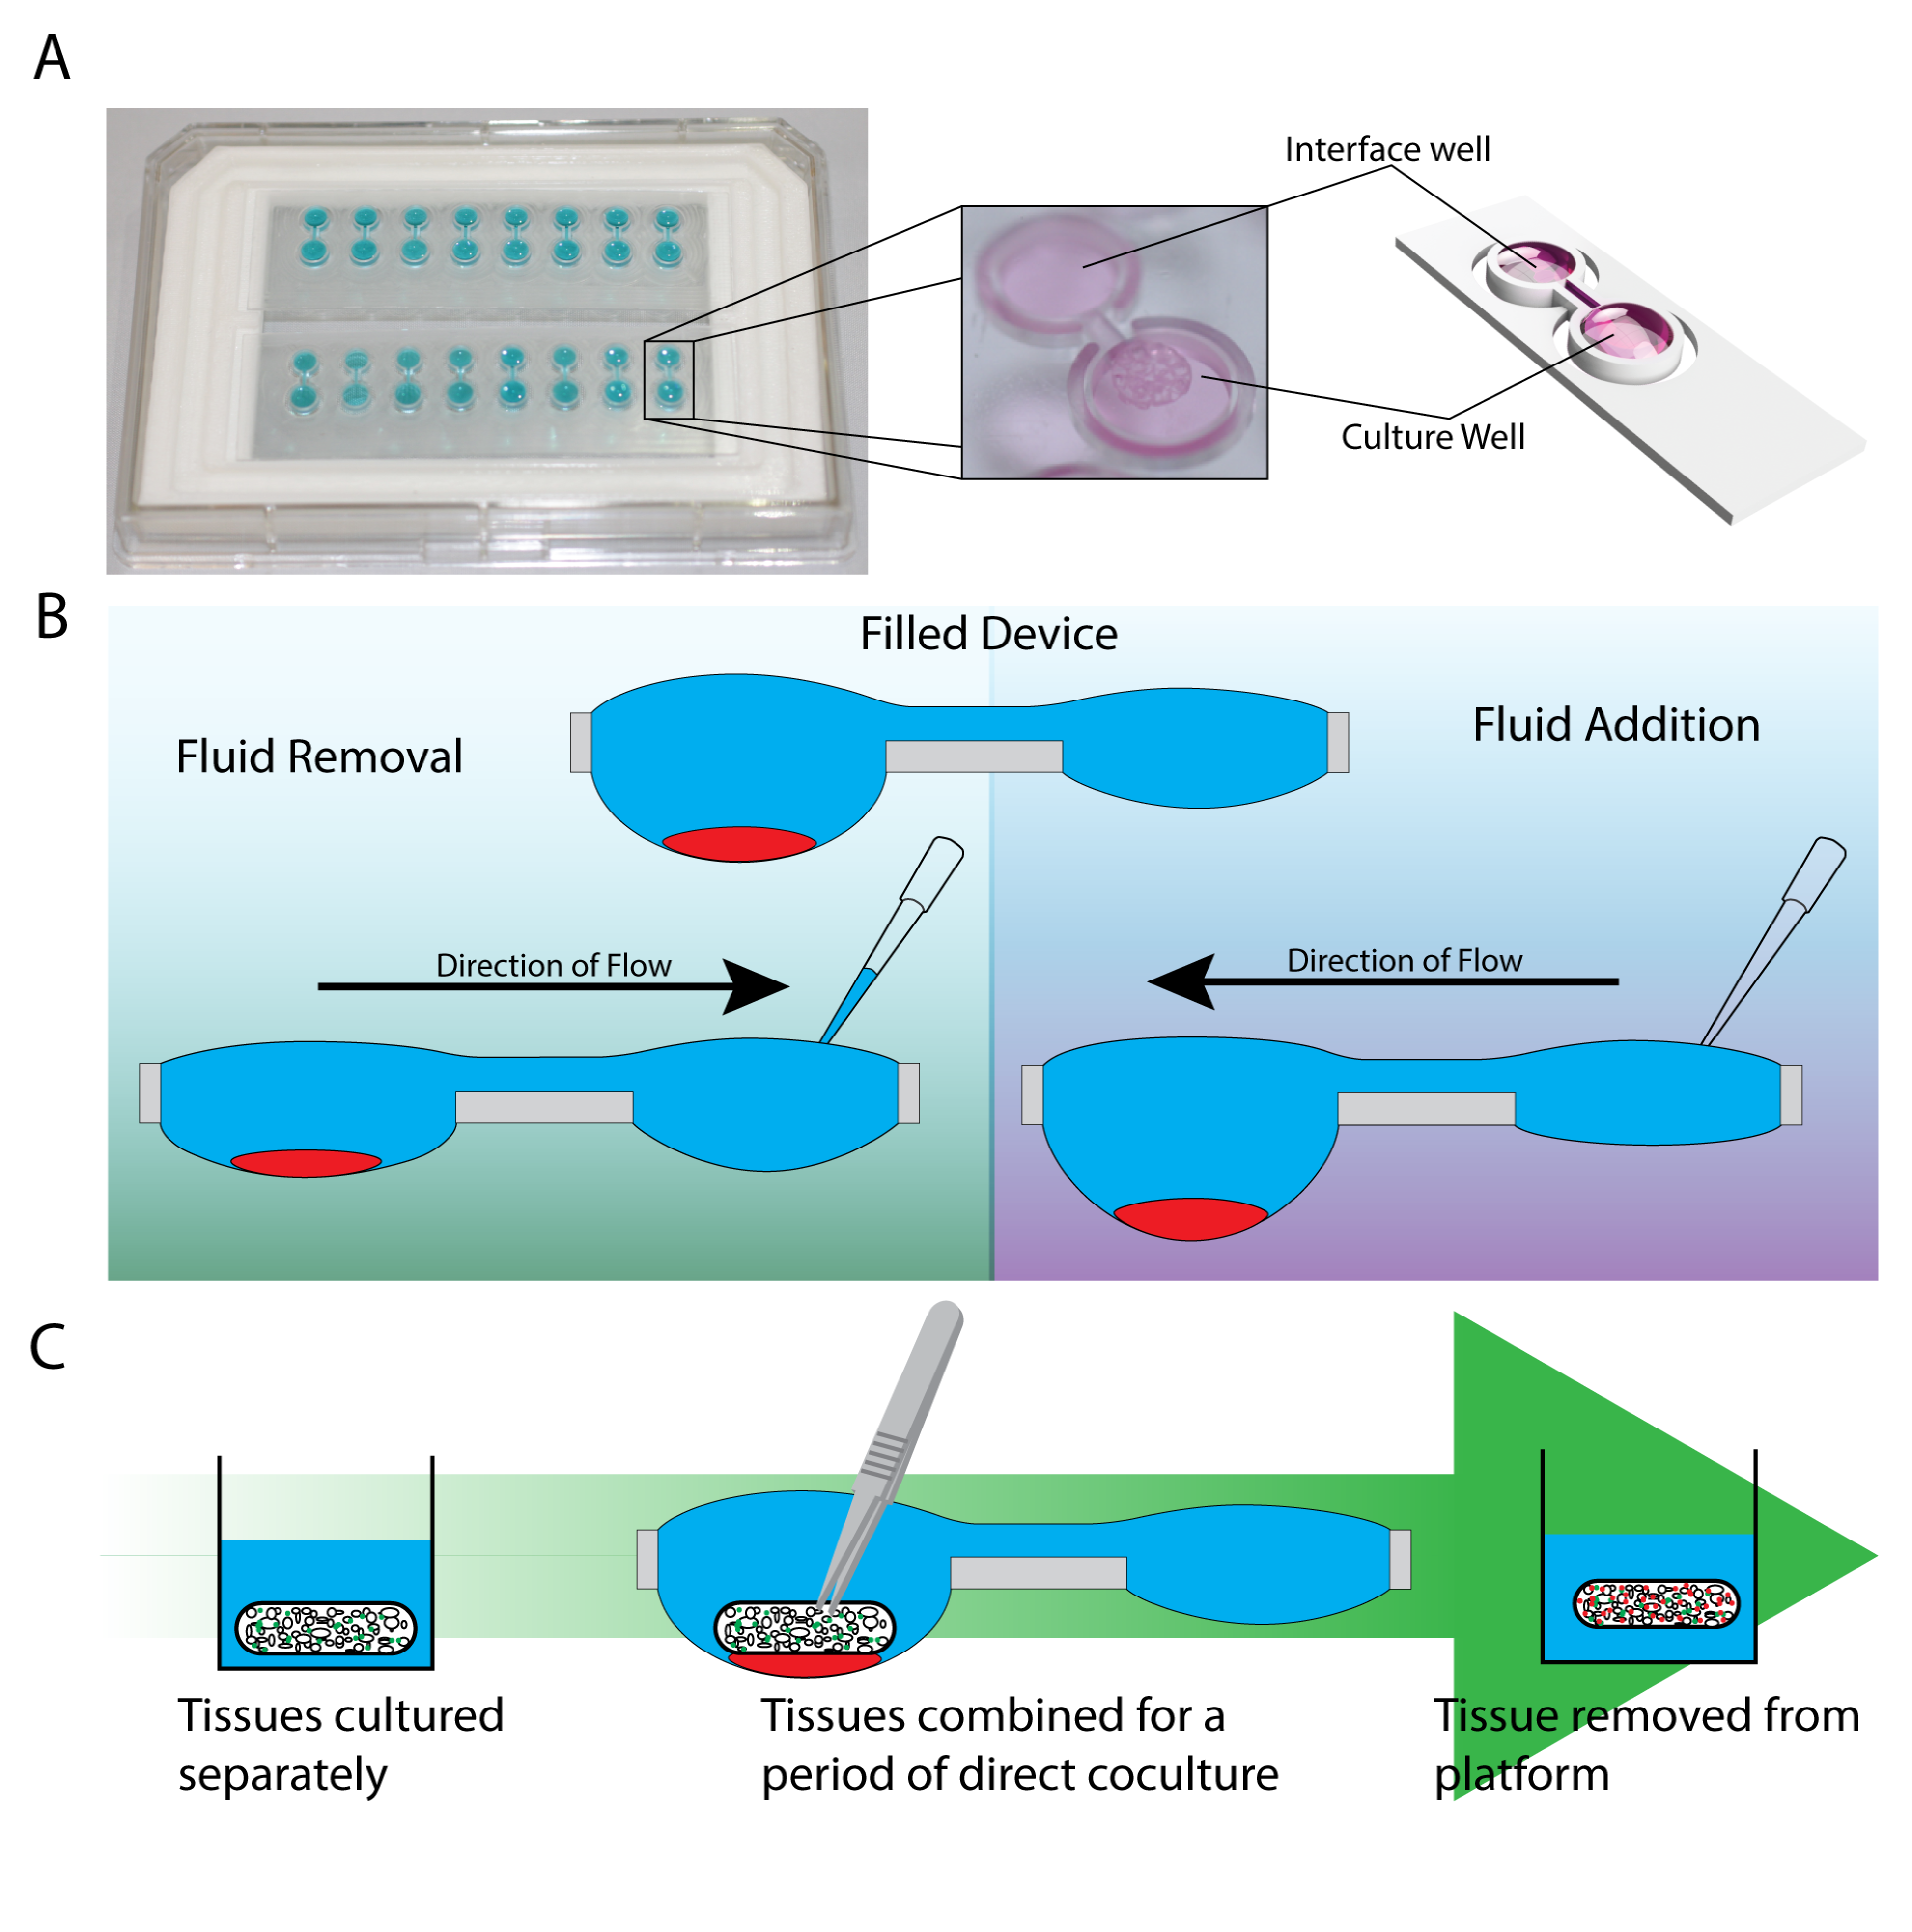
\includegraphics[width=5.4in]{/Figure1-RSC.png}
\caption[\textbf{The two-well hanging droplet device, operation, and capabilities}]{\textbf{The two-well hanging droplet device, operation, and capabilities}. (A) Two 8- device arrays of the two-well hanging droplet device with a close-up image and rendered-model of a single device. (B) Operation of a filled device containing cells, when fluid is removed or added through the interface well, volume of the culture well is changed with minimal disturbance to the culture. (C) Schematic of a dynamic coculutre experiment performed by combining two tissues in the hanging droplet device then separating the tissues.}
\label{figure:Fig1}
\end{figure}


\subsection{Characterization and modeling of two-droplet system}
We developed a numerical model for the behavior of the connected two droplet system to understand the limitations of the system, improve the functionality of the system, and guide the design of suspended droplet systems. The model predicts the distribution of fluid between two droplets as fluid is added or removed from the system. These predicted values were compared to values experimentally acquired in the device (Fig. \ref{figure:Fig2}Ai). Having a range of well characterized values allows the operation of the device with volumes that are robust and do not risk potential modes of failure. At low volumes, the hanging drop follows a surface-tension dominant regime dictated by the Laplace pressure \cite{Walker2002, Berthier2007} in which the two drops are close in volume. At higher volumes, however, gravity is non negligible, and the shape of the drop becomes elongated \cite{Carvajal2011}. Fluid distribution between wells at increasing volumes is illustrated in Figure \ref{figure:Fig2}Aii where the modeled fluid borders of each well at each volume is overlaid on images of the device. 

To predict the behavior of the system during device operation, we created a dynamic model of the device (Fig. \ref{figure:Fig2}B). With the model, we are able to observe that when one of the droplets, typically the droplet in the largest suspended port, becomes the lowest pressure region it acquires the majority of the liquid in the system. The model further shows that adding and removing fluid to the small drop results in approximately the same volume being shuttled to the well containing the largest drop. Importantly, this model validates the use of the small drop as a buffer for fluid additions; the small drop temporarily stores the fluid that was added by pipetting, prior to delivering it to the larger drop. Utilizing this approach, it becomes simple to tailor the delivery rate to the large drop in order to prevent excessive flow by designing the geometry of the channel connecting the two drops appropriately \cite{Berthier2011}. Finally, the model incorporates the dripping volume for a hanging drop, allowing the prediction of the maximum volume that can be added before detachment of the large drop. Alternatively, this can be utilized as a method for collecting the cellular sample; precise volumes of fluid can be added to cause the dripping of the cells in the drop into a receptacle placed below.

\begin{figure}[h!] %DONE
\centering
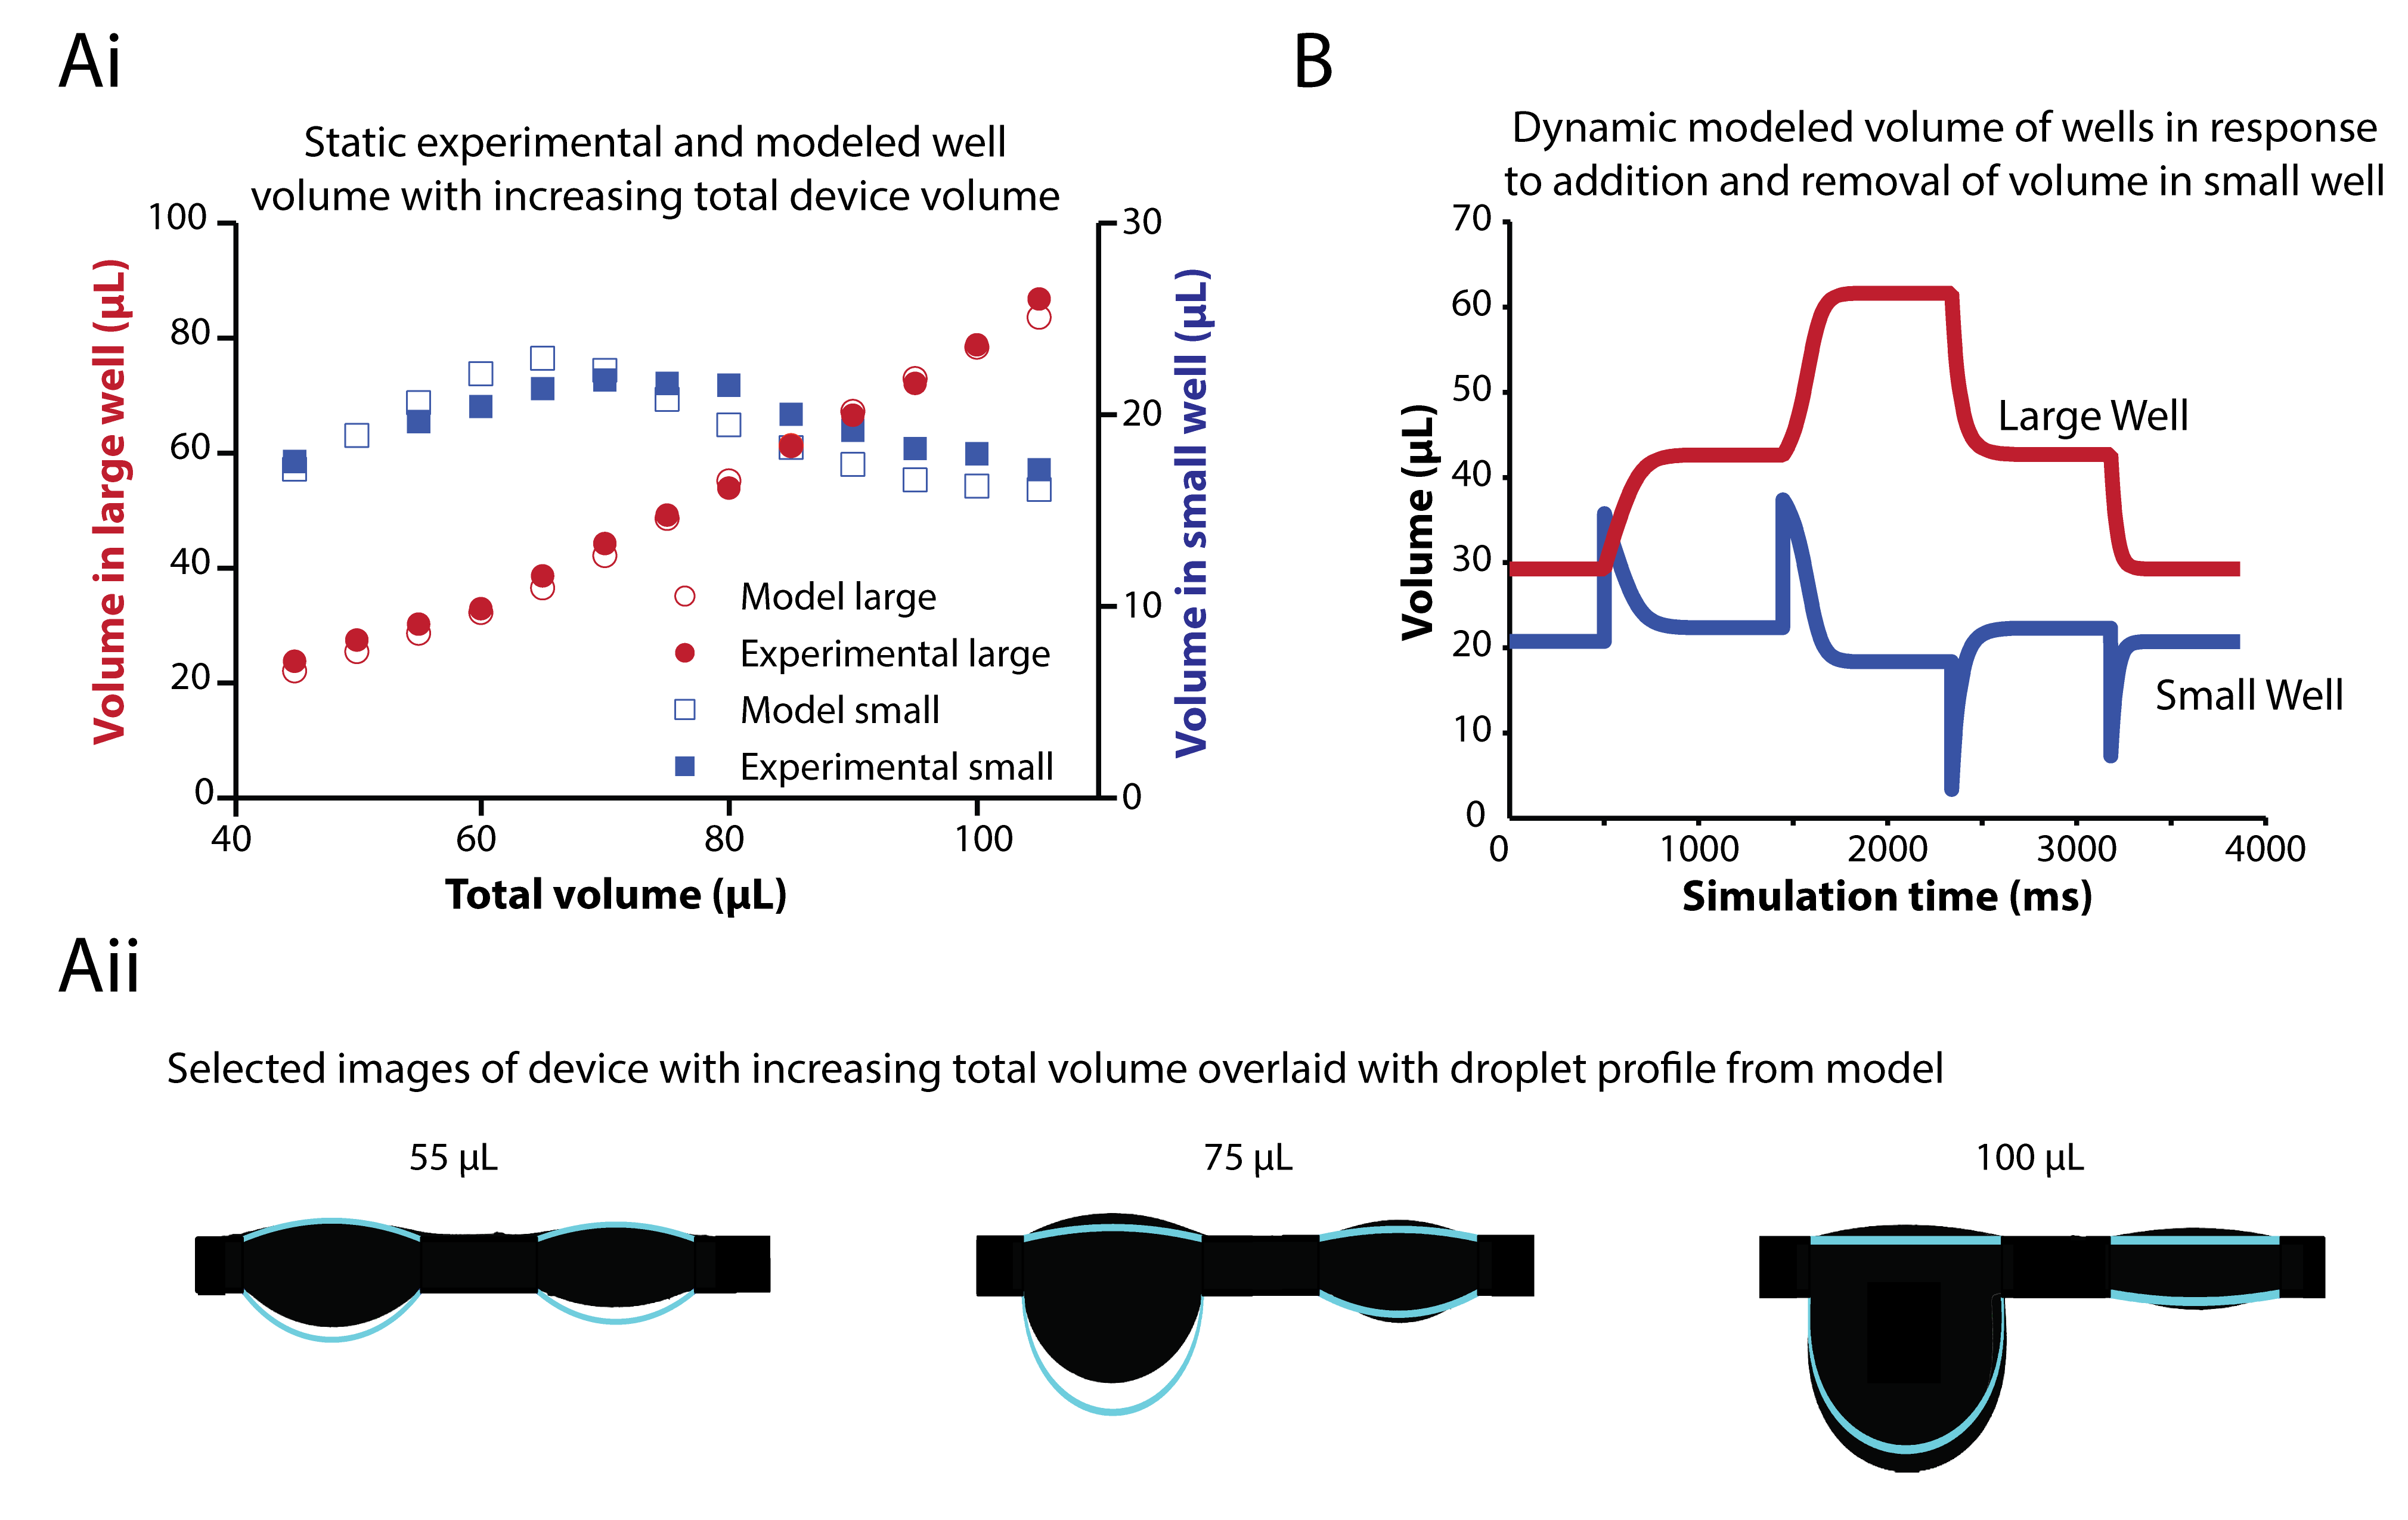
\includegraphics[width=5.75in]{/Figure2-rsc-01.png}
\caption[\textbf{Static and dynamic modeling of volume in each well of the device.}]{\textbf{Static and dynamic modeling of volume in each well of the device.} (Ai) The experimental (solid) and modeled (hollow) volume in each well at steady state with increasing total volume in the device. (Aii) The silhouetted device overlaid with the droplet borders of the modeled system for 55, 75, and 100 μL of total fluid in device. (B) Dynamic modeling of fluid in each well of the device as fluid is added then removed from the small well.}
\label{figure:Fig2}
\end{figure}


\subsection{Two-well hanging drop system prevents shear stress during media exchange}
Shear stress on a cell results in considerable changes to cell behavior \cite{White2007}, including inhibition of apoptosis in some cells \cite{Dimmeler1996} and induced proliferation and differentiation in other types \cite{Yamamoto2003}. In spheroid culture shear can prevent aggregation and completely disrupt the macrostructure of suspension cell cultures. Reducing shear experienced by cells in culture is critical to minimizing undesirable cell stimuli and achieving consistency between experiments. The two-well system provides a reduction in shear stress when changing fluid in hanging droplets compared to a one-well system. We performed an experiment to determine the extent of protection provided by the damping effect for droplet equilibration observed in our model (Fig. \ref{figure:Fig2}). This is best illustrated by a direct comparison between the two- and one-well systems (Fig. \ref{figure:Fig3}). We chose a multiple myeloma suspension cell line, MM.1S (commonly used for multiple myeloma drug studies \cite{Greenstein2003, Tai2006, Azab2009}) for the comparison, because suspension cell lines are generally difficult to culture in microdevices and are easily removed by flow. When cultured in the hanging droplet platform, MM.1S cells settle into clusters but do not form sphereoids. Addition or removal of fluid will result in loss of myeloma cells since the cluster is easily disturbed by minimal force exerted during fluid manipulation. In the hanging drop system media replacement is performed using iterative pipetting steps. Thus, we compared the performance of the two- and one-well systems over multiple pipetting steps.

We designed the experiment to ensure accurate comparison between the two- and one-well systems. The diameter and volume of the culture well in the two-well and one-well system was identical; the volume of fluid removed was based on a fraction (one third) of the total volume in each system. Pipetting was performed by a liquid handling robot to keep the flow rate constant. Each image in Figure \ref{figure:Fig3}A represents a different well subject to different conditions of fluid exchange, and all well images were collected within 10 minutes of pipetting. The two-well system protects cell clusters during fluid exchange after several pipetting steps, while pipetting into the one-well system results in immediate disruption of cluster morphology. These results combined with the data generated from computational modeling of the system underscore the need for an unequal two-well system for suspension cell culture to culture and retain cells to a single well, and suggest that media exchanges in one-well systems may have unintended effects on suspension cell culture.

To evaluate the difference in shear between pipetting into a single-well versus a two-well system, we performed particle image velocimetry (PIV) analysis on fluorescent microbeads in the culture well (Fig. \ref{figure:Fig3}B). Fluid was added \textit{via} the user interface well (in the two-well system) or directly into the culture well containing the fluorescent beads (in the one-well system). There was a 10-fold reduction in the velocity of beads in the two-well device compared to the single-well one. This reduction velocity corresponds to a comparable decrease in shear stress experienced by cells in the device. Furthermore, the reduction in velocity in the two-well system enables quicker media changes without cell disruption, compensates for variation of users operating the device manually, and results in shorter times where the device needs to be exposed (to interface with pipettes), reducing potential evaporation.

\begin{figure}[h!] %DONE
\centering
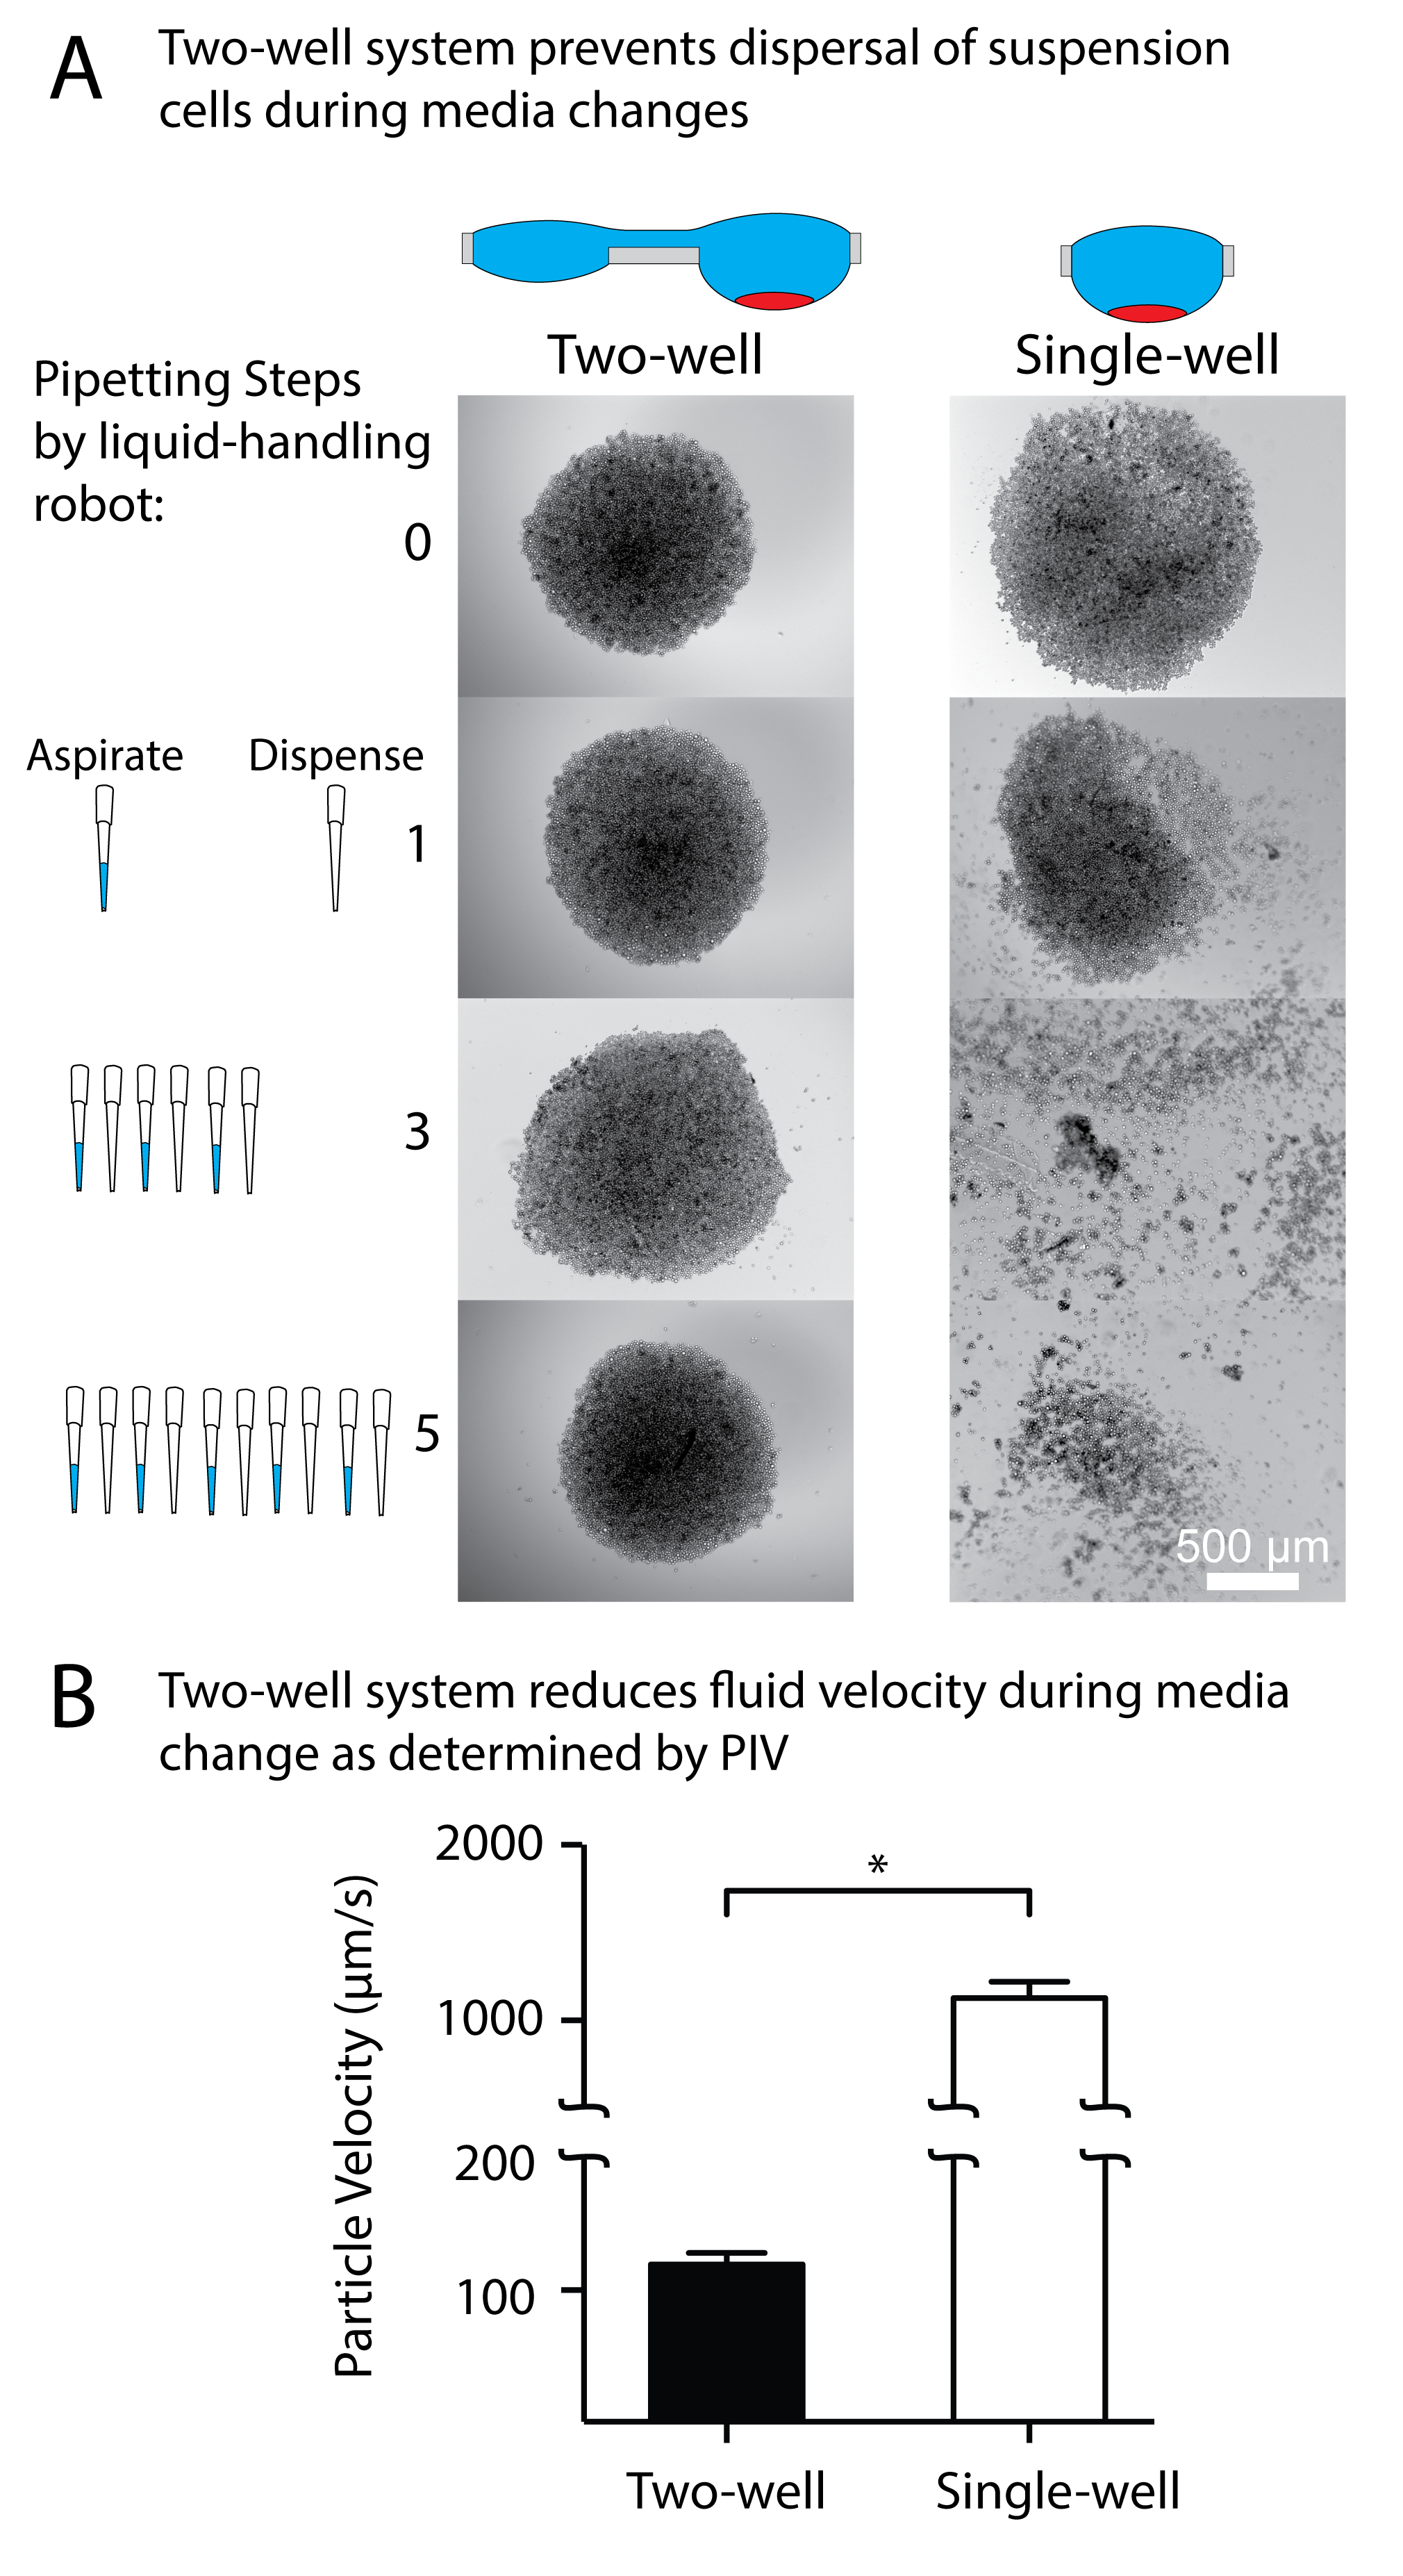
\includegraphics[width=3in]{/Figure3-RSC.png}
\caption[\textbf{Effects of pipetting into a single-well and two-well device}]{\textbf{Effects of pipetting into a single-well and two-well device.} (A) Brightfield images of an MM.1S suspension culture in the device before and following 1, 3, and 5 pipetting steps at 1 mL/min of approximately 33\% of the total media in single-well and two-well device. (B) PIV was used to determine the velocity of fluid at a fixed z position in the culture droplet during fluid addition to the interface droplet (two-well) or directly (single-well). Error bars represent the standard deviation of four replicates (*p<0.0001).}
\label{figure:Fig3}
\end{figure}

\subsection{Open hanging droplet platform facilitates key cell culture manipulations and readouts}
For functional validation, we demonstrated that the hanging droplet culture platform is well suited to perform functions critical for tissue culture, experimentation, and analysis: long-term culture, ability to apply treatment, and immunocytostaining. We chose to focus our cellular validation experiments using suspension (or non-adherent) multiple myeloma cells. Multiple myeloma is the second most common hematopoietic malignancy in the United States, and has a 47\% median 5-year survival rate. Multiple myeloma affects its microenvironment through a complex network of interactions with surrounding matrix and cells resulting in the destruction of healthy bone \cite{Reagan2014} and acquisition of drug resistance \cite{Bianchi2006}. The fact that multiple myeloma cells are non-adherent precludes the use of many currently available microculture platforms for studying the disease.  We performed the platform validation using the multiple myeloma cell line, MM.1S. The MM.1S cell line is an important model for multiple myeloma, and the assays we have focused on are key to studying the disease and patient-specific drug responses \cite{Young2012}.
\newline
\textit{i. Long term culture.} The extended culture experiments were performed over the course of 9 days, feeding the culture every other day through media replacements, resulting in approximately 75\% new media in the culture well each feeding. The MM.1S cells expressed mCherry, which was used to perform a relative quantification of total cells in the well. Mean integrated density of fluorescence signal across the entire well was used because a single cell count was not feasible due to the high density of cells and cell-to-cell variation in mCherry expression levels. Over the course of the experiment (Fig. \ref{figure:Fig4} A), the number of cells increased through day 5, but had stopped by the 6th day. At that time in the culture, the wells had become overpopulated resulting in stagnation of the mean integrated density. Though nine-day culture is rarely required for common experiments such as drug screens, we have demonstrated the practicality of long-term culture in the device. \newline
\textit{ii. Cell viability in response to \textit{in situ} treatment.}

We characterized growth inhibition of the culture in response to a drug to demonstrate the ability to apply treatments during culture and measure a dose-response. We treated MM.1S cells with bortezomib, a proteasome inhibitor and commonly used treatment for multiple myeloma (Fig. \ref{figure:Fig4}B). The IC50 value of the MM.1S culture in response to bortezomib was determined to be 26.2 nM with an R\textsuperscript{2} of 0.84. The previously reported IC50s of bortezomib for the MM.1S cell line typically range between 4 and 9 nM \cite{Bianchi2006, Hu2014, Horton2006}, but these values were all calculated in 2D culture. It has been widely shown that 3D culture conditions often decrease drug sensitivity \cite{Tung2011, Friedrich2009}and better recapitulate in vivo response. The calculated response also for a 24 hour exposure time, follows a distinct 4 parameter logistic sigmoidal curve characteristic of inhibitory dose-response curves. 

\textit{iii. High content assays and immunocytochemistry (ICC)} To establish the viability of functional readouts in the platform, we characterized NF-\textkappa B translocation to the nucleus in MM.1S cells in response to stimulation \textit{via} TNF-\textalpha. Quantifying translocation of factors between cell membrane, cytoplasm, and nucleus of the cell provides a high-content assay that can give information about the state of a single cell or population of cells. Translocation of factors around the cell is a vital component in cell behavior and proliferation \cite{Chuderland2008}. Misregulation of translocated factors, such as estrogen receptor in breast cancer \cite{Revankar2005} and androgen receptor in prostate cancer \cite{Molina2011}, contributes to treatment resistance. In multiple myeloma, NF-\textkappa B has been implicated as key regulator of inflammation, cancer progression, cell survival, and acquired resistance \cite{hideshima2000thalidomide}, and thus is considered as a potential therapeutic target. 

We performed an experiment to induce translocation of NF-\textkappa B in response to TNF-\textalpha  in the MM.1S cell line (Fig. \ref{figure:Fig4}C). TNF-\textalpha  is expected to cause NF-\textkappa B to translocate to the nucleus following treatment and is the first step in the transcription of a number of pro-inflammatory mediators \cite{Pahl1999}. Translocation is indicated by a steeper slope in the scatter plot comparing the mean signal intensity of NF-\textkappa B in the nucleus versus the cytoplasm (Fig. \ref{figure:Fig4}Ci). When considering the entire population of cells using a histogram, a population-wide increase in translocation is visualized as a shift to the right on the x-axis (mean nuclear NF-\textkappa B signal intensity to mean cytoplasmic NF-\textkappa B signal intensity) with a median shift from 1.0 in the untreated condition to 1.2 in the treated conditions with p<0.001 from analysis with the Mann-Whitney U test for 4 replicates (Fig. \ref{figure:Fig4}Cii).

\begin{figure}[h!] %DONE
\centering
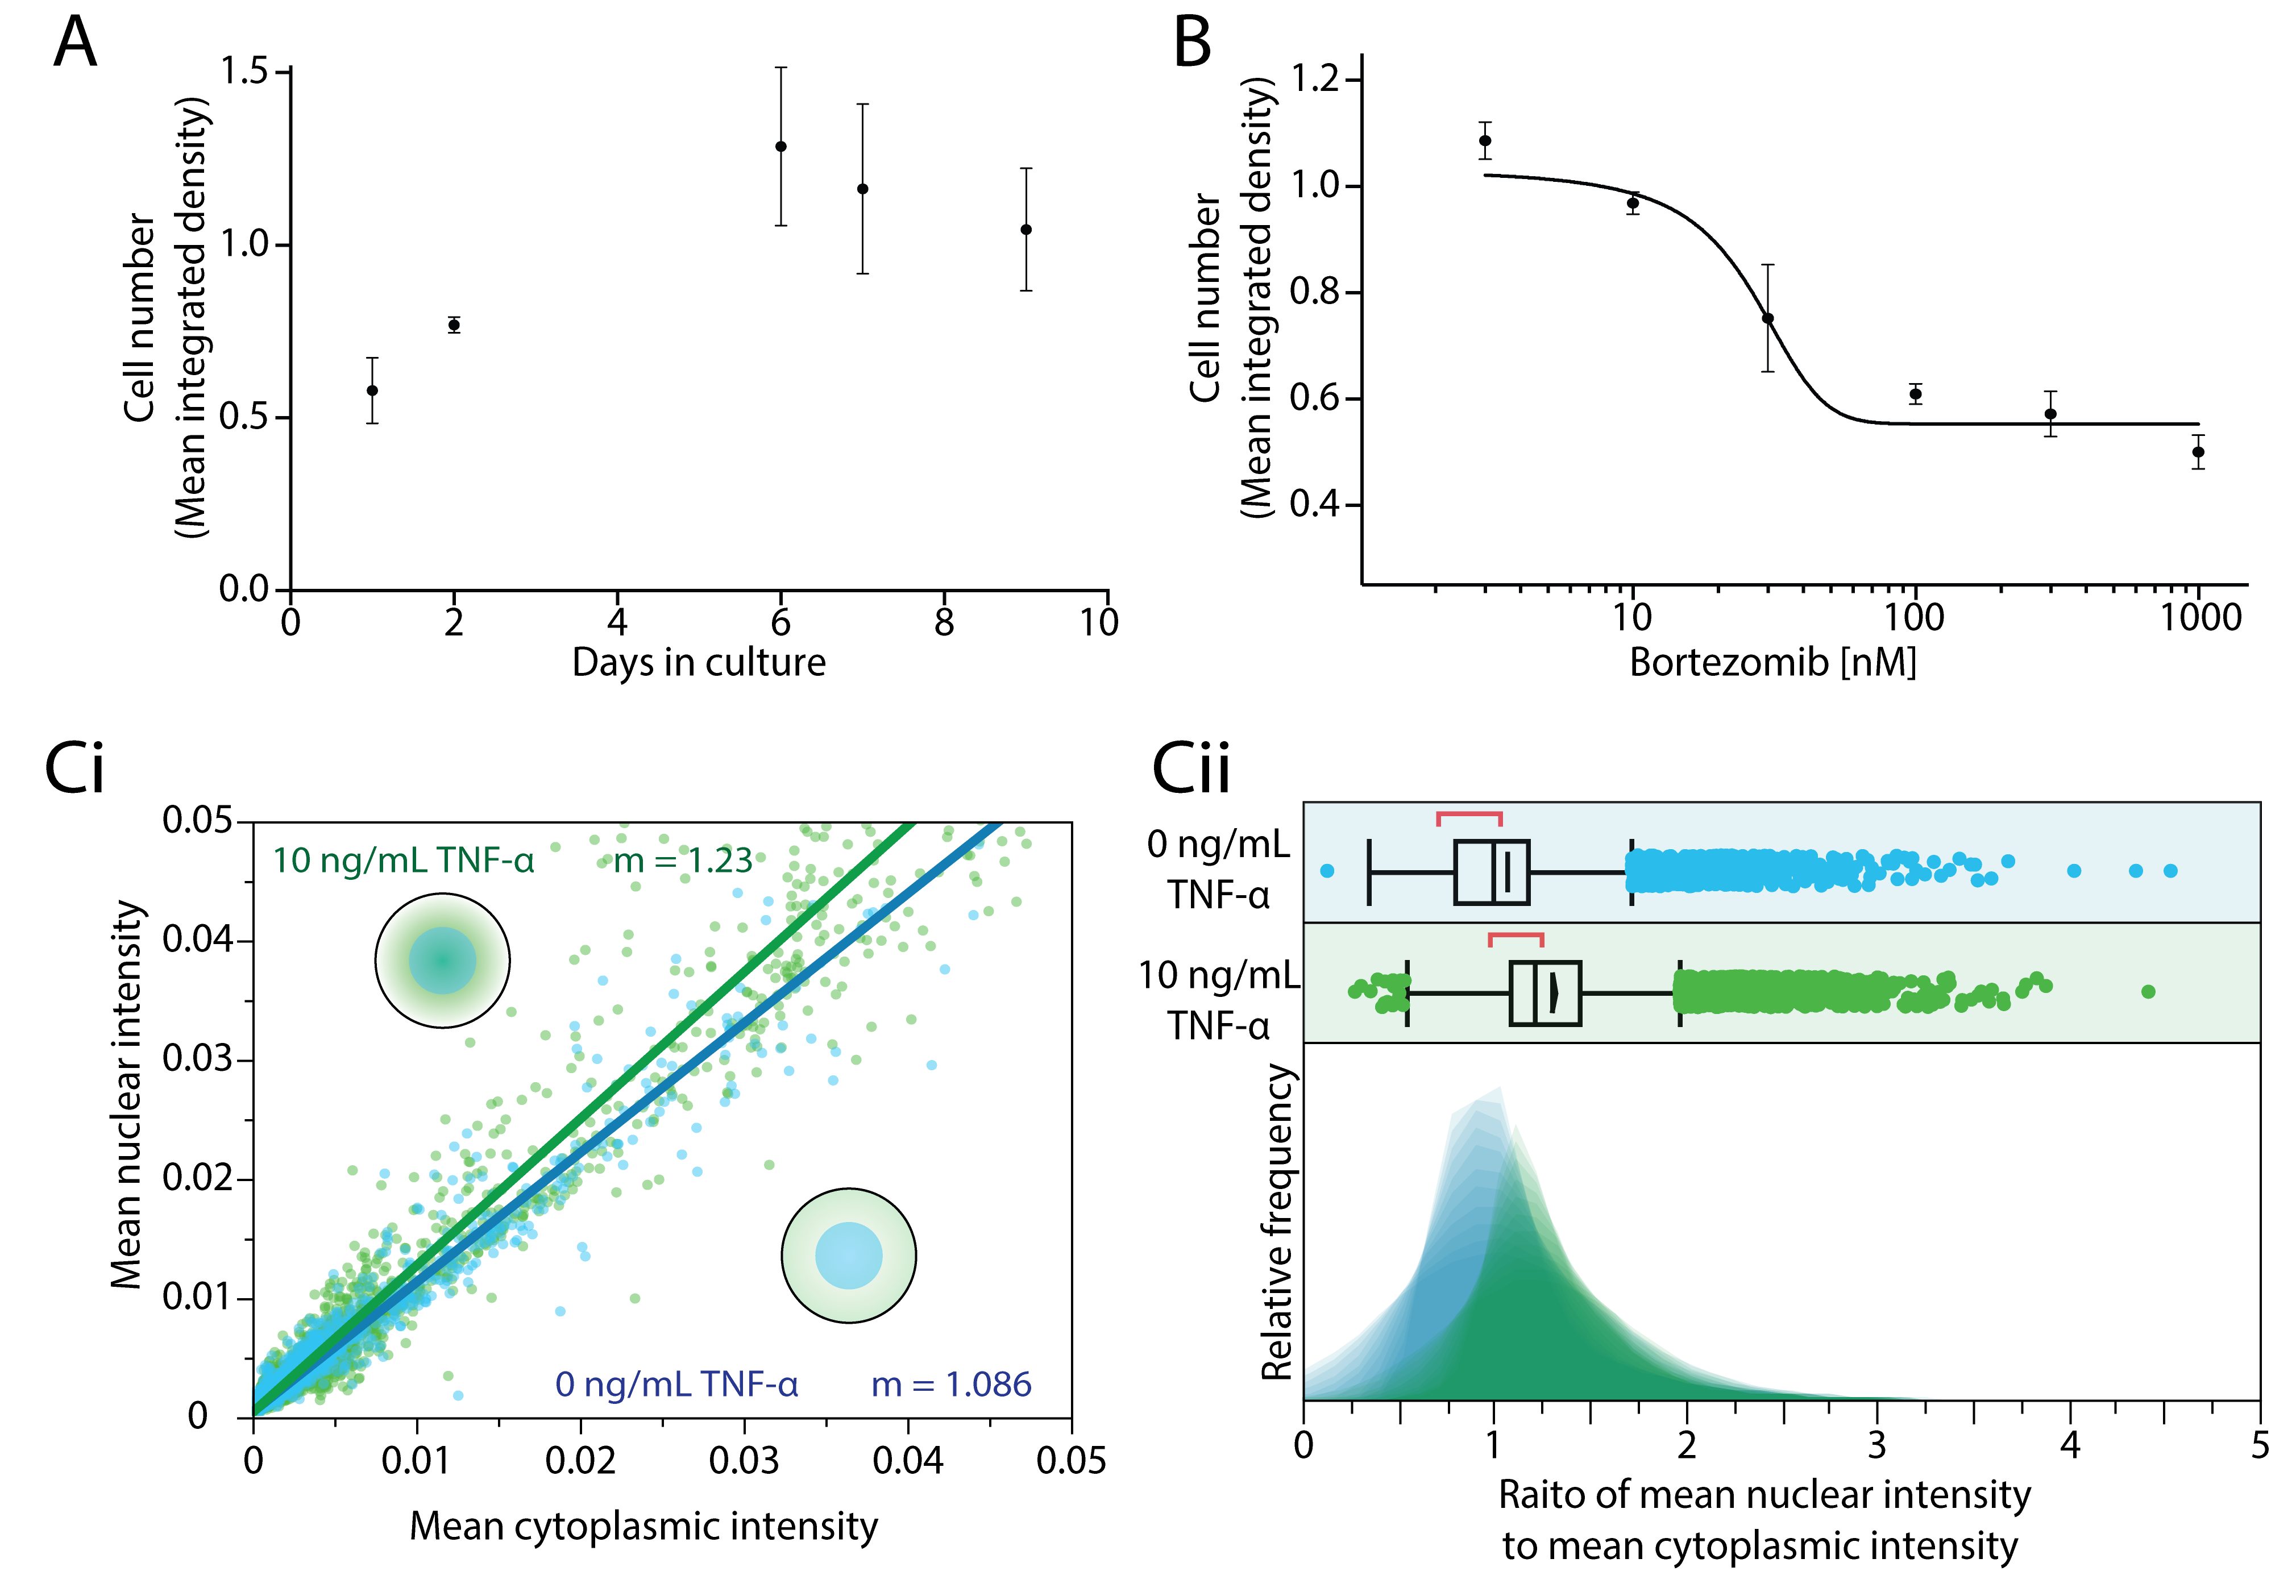
\includegraphics[width=5.75in]{/Figure4-RSC.png}
\caption[\textbf{Open hanging droplet platform facilitates key cell culture manipulations and readouts.}]{\textbf{Open hanging droplet platform facilitates key cell culture manipulations and readouts.} (A) Long term culture: Growth of MM.1S cells in device across a 9-day culture. Error bars represent the standard error of the mean (SEM) of 7 wells. (B) Cell viability assays in response to in situ treatment: Growth inhibition response curve of MM.1S cells to increasing concentrations of bortezomib in culture. Error bars represent the SEM of 5 wells. (C) Characterization NF-\textkappa B nuclear translocation in MM.1S cells following treatment with 10 ng/mL of TNF-\textalpha \, (green) or no treatment (blue). (Ci) Scatter plot of mean nuclear intensity versus mean cytoplasmic intensity. (Cii) Histograms of the ratio of mean nuclear intensity to mean cytoplasmic intensity for the population of cells.}
\label{figure:Fig4}
\end{figure}

For the NF-\textkappa B translocation assay described above, we developed methods to perform ICC on cells from hanging drop cultures. We first attempted to perform ICC in situ (i.e., in the hanging droplet device), leveraging the two-well system to exchange ICC reagents. However, performing ICC requires a permeabilization step using surfactants, which inherently reduce interfacial tension. Standard in situ ICC was found to be incompatible with the hanging droplet device due to the reliance on pressure equilibration to move fluid between wells. When surfactant is added to the user interface well  the surface tension decreases, causing a shuttling of fluid from the culture well into the interface well. To achieve high-content ICC in the NF-\textkappa B translocation assay, we instead transferred the cells from the hanging droplet wells to a poly-L-lysine-treated slide to retain cells during fluid exchange by touching off the droplets onto the surface of the slide.  Performing ICC and imaging on plated cells has several advantages compared to in situ ICC and imaging. The cells are spread throughout the plate, allowing for better separation of cells and therefore better characterization of single cells to be achieved. Plating cells also enables higher objectives to be used for imaging and longer imaging times to be achieved. In the current configuration, devices would need to be removed from the humidifying dish to be accessed by high magnification objectives due to working distance limitations. 

It is worth noting that other staining protocols that do not require surfactants, such as live/dead assays, can be performed directly in the hanging droplet device. We demonstrated this using the adherent cell line MDA-MB231, which forms spheroids in hanging droplet culture (Fig. \ref{figure:FigS2}). We incubated the device in both normoxic and hypoxic conditions to study the spatial distribution of live and dead cells within the spheroid. Live/dead staining was performed within the hanging droplet device, and the spheroids were removed for imaging (Fig. \ref{figure:FigS2}). 
\newline
\textit{iv. Culture treatment, media sampling and cytokine quantification}The ability to sample and analyze media throughout the course of an experiment without disturbing the culture is powerful for studying progression of a culture system. The two-well system is well-suited for media collection and treatment addition through the interface well. To validate the platform for treatment and sampling, we cultured a polymeric porous bone-like scaffold seeded with bone marrow stromal cells in the device. The scaffolds were treated at seeding and after 24 hours with AMD3100, an inhibitor of CXCR4, indicated in homing and adhesion for cells to the bone marrow microenvironment \cite{Alsayed2007, Burger2006}. The media was sampled at 24 and 48 hours from the interface port and analyzed for the pro-inflammatory, IL-6 cytokine indicated in microenvironment-mediated drug resistance and a number of pro-tumorigenic pathways \cite{Hodge2005, Roodman2001a, Vincent2005, Lin2007}. IL-6 was detected in both the control and AMD3100-positive conditions when sampled from the interface well (Fig. \ref{figure:Fig5}A). As expected, we observed a trend toward reduced IL-6 secretion with AMD3100 treatment. This experiment demonstrates that cytokines secreted by cells in the culture well are able to be detected in the interface well and suggests that this device could provide a useful tool for conducting soluble factor signaling-based coculture experiments using more complex culture constructs. We further evaluated soluble factor exchange in the device through computational modeling of diffusion in the system starting with an initial concentration of a molecule with similar diffusion properties to IL-6 in the volume occupied by the bone-like scaffolds (Fig. \ref{figure:Fig5}B). At 4 hours, the diffusion gradient stabilizes within the culture well of the device creating a pattern where the culture well has a stable "high" concentration and the interface well have a stable "low" concentration of the solute. Further characterization of diffusion within the device is available in the ESI (Fig. \ref{figure:FigS3}).    

\begin{figure}[h!] %DONE
\centering
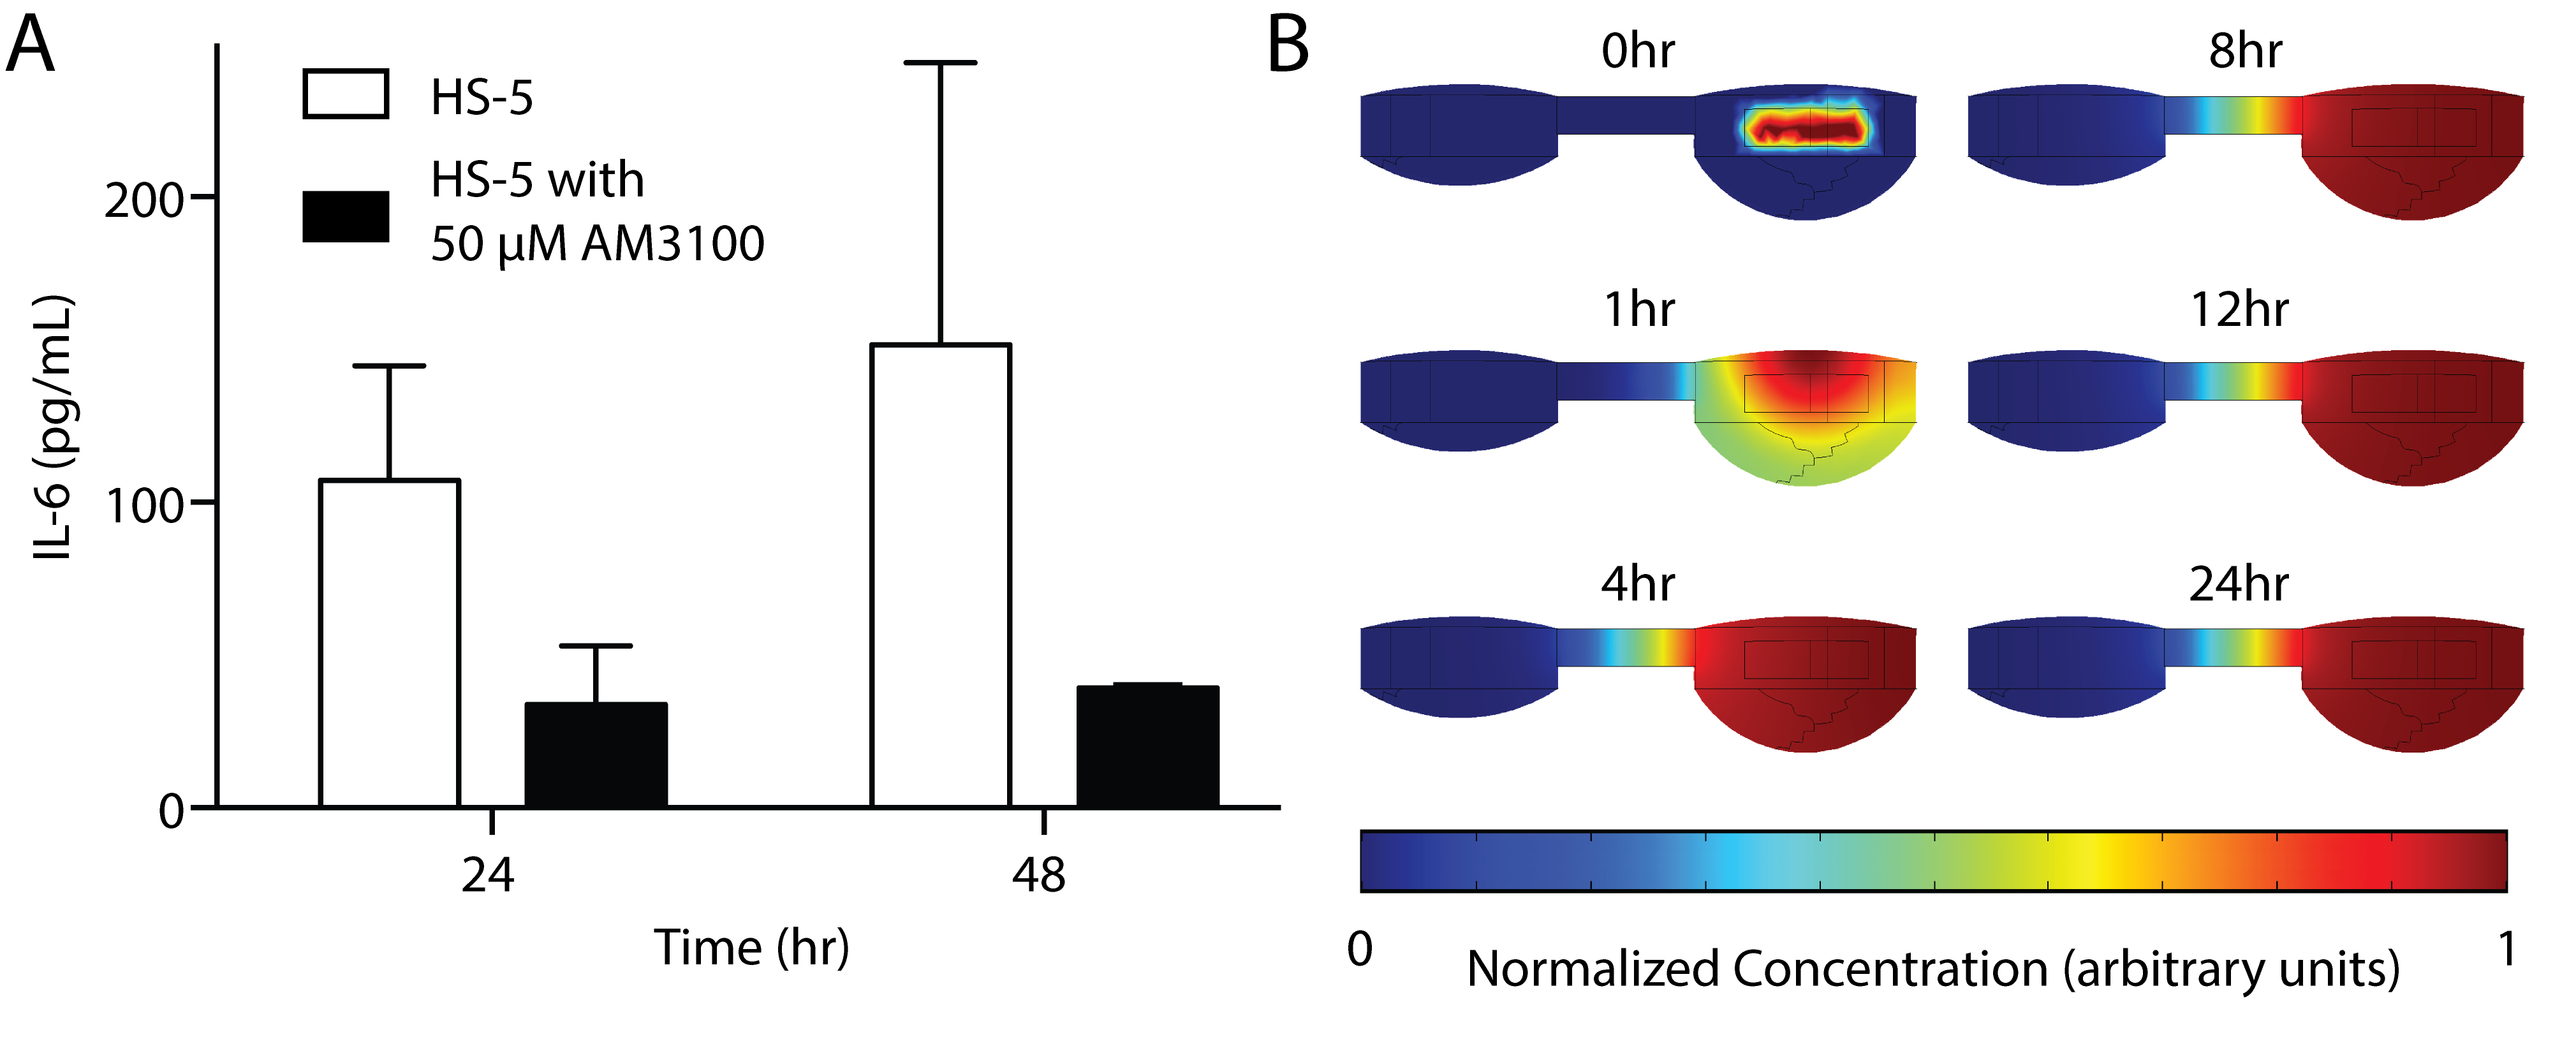
\includegraphics[width=5.75in]{/Figure5-RSC.png}
\caption[\textbf{Soluble factors in culture.}]{\textbf{Soluble factors in culture.} (A) Concentration of IL-6 isolated from HS-5-seeded bone-like scaffolds cultured in device taken from the interface well at 24 and 48 hours of culture. Error bars represent the SEM of 3-4 wells. (B) Plot of normalized concentration for simulated diffusion in the device at several time points over 24 hours. The initial concentration of solute was localized to the volume occupied by the bone-like scaffold at time = 0 h. The solute simulated was approximately 10 kDa with a diffusion coefficient of 100 \textmu m\textsuperscript{2}/s.}
\label{figure:Fig5}
\end{figure}


\subsection{Dynamic culture of cells and tissue scaffolds}
The geometry of the device allows for direct access to the culture through the open wells. This access can be exploited to manipulate culture throughout the course of an experiment. We demonstrated manipulation of the media through the wells (sections 3.3 and 3.4), importantly, the open system facilitates interaction beyond simple media changes and liquid treatments. As shown in Fig. \ref{figure:Fig1}, tissue scaffolds and solid objects can be introduced \textit{via} direct access to the culture well (e.g., by using tweezers to place the scaffold in the open device). To explore the ability to manipulate tissue throughout the course of an experiment, we performed a coculture of multiple myeloma and bone marrow stromal cells (BMSCs). BMSCs play an important role in multiple myeloma progression and provide the tumor with protection against treatment \cite{Chauhan1996, Chatterjee2002a}. Adhesion of multiple myeloma cells to the stroma is an important step in disease progression as non-malignant B-cells have very low capacity for adhesion \cite{Tai2006}.

We began the culture separately, with BMSCs in polymeric, porous, bone-like scaffolds and myeloma seeded into wells in the hanging droplet device. The cultures were combined in the hanging droplet device and myeloma cells were allowed to migrate into the scaffold. The scaffolds were removed for imaging following coculture and adhesion of MM.1S cells was characterized (Fig. \ref{figure:Fig6}). Adhesion of the MM.1S cells to the scaffold was seen in both direct coculture, where the scaffold and MM.1S cluster were in the same well, as well as in the blank scaffold MM.1S monoculture condition. MM.1S cells were not detectable in either BMSC monoculture or separate coculture. These results enable us to explore the impact of the multiple myeloma microenvironment for both soluble factor signaling as well as cell-cell contact for tumor-stromal interactions. 

\begin{figure}[ht] %DONE
\centering
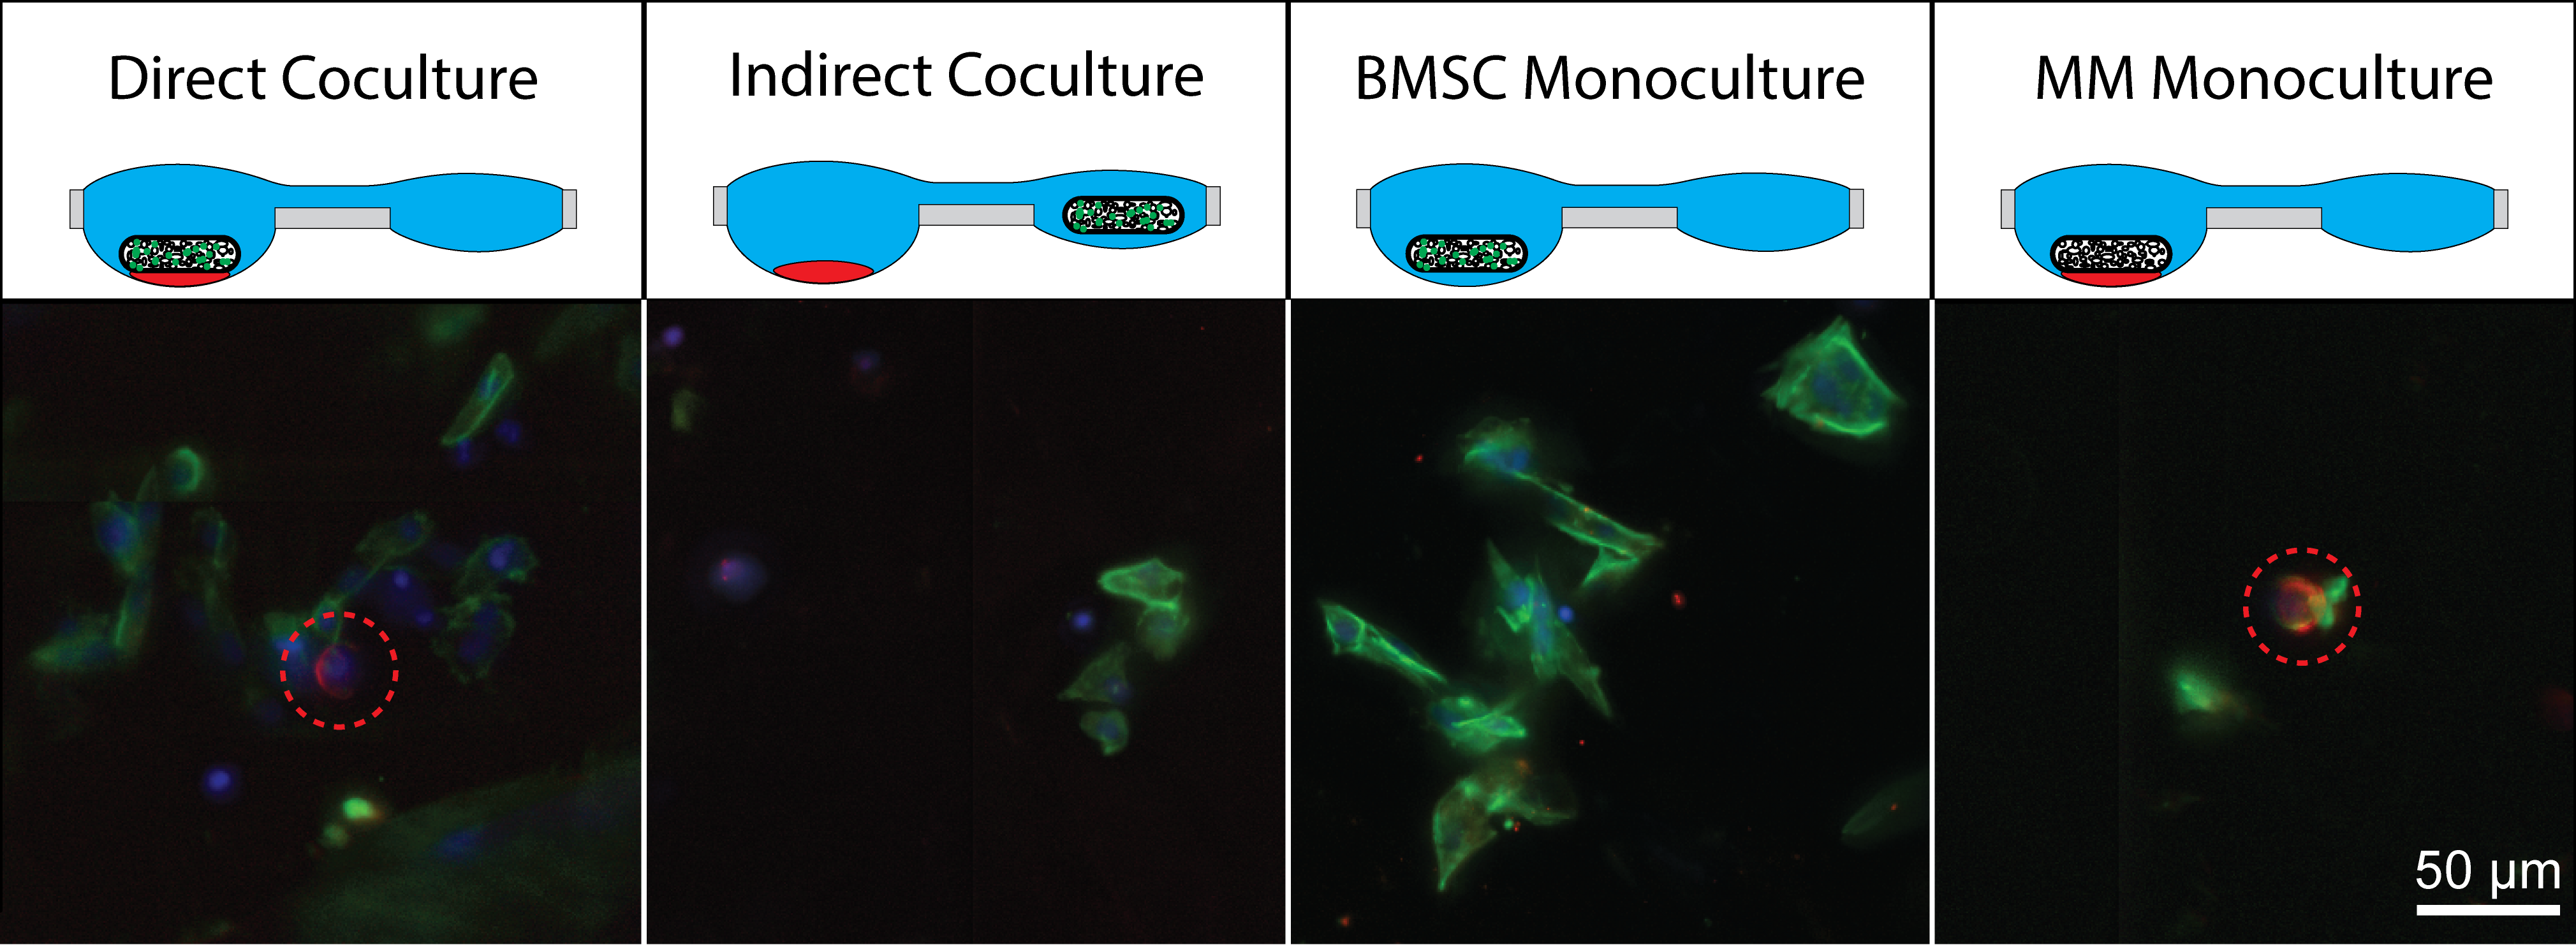
\includegraphics[width=5.5in]{/Figure6-RSC.png}
\caption[\textbf{Coculture and migrations of MM.1S cells into polymeric bone-like scaffold.}]{\textbf{Coculture and migrations of MM.1S cells into polymeric bone-like scaffold.} Fluorescent images of polymeric bone-like scaffolds following either direct coculture (BMSC-seeded scaffold with MM.1S cluster - same well), indirect coculture (BMSC-seeded scaffold with MM.1S - separate wells), BMSC monoculture (BMSC-seeded scaffold only), or multiple myeloma monoculture (MM.1S cultured with blank scaffold). BMSCs were identified by presence nuclear stain (blue) with actin (green), while MM.1S cells were identified by nuclear stain, actin, and CD138 ring (red) and highlighted with a red dotted circle.}
\label{figure:Fig6}
\end{figure}


\section{Conclusions}
We have developed an open platform that enables the dynamic culture and analysis of tissues in a hanging drop embodiment. We have demonstrated that an asymmetric two-well droplet system enables the long-term culture of shear-sensitive cells while allowing for the application of treatments over the course of an experiment. Leveraging the open surface of the hanging drop wells, we are able to add and remove tissue from the culture platform during the course of an experiment to enable dynamic coculture configurations, which are difficult to achieve in closed culture platforms and facilitates easy downstream analysis of cultures. The platform addresses challenges of culturing suspension cells in 3D culture as well as coculture with adherent cell types. The platform enables configurations of cells that were previously either unachievable or impractical, allowing for the investigation of new biological phenomena. We will continue to explore the biology enabled by this platform with the development of more complex biological tissues formed with step-wise, dynamic component addition. 

\section{Acknowledgements}
The authors would like to thank Drs. Shigeki Miyamoto and Fotis Asimakopoulos for their expertise and biological insight into multiple myeloma, Dr. William Murphy and Eric Nguyen for their contributions to in situ imaging in the  and bone marrow scaffold development, and Dr. Jay Warrick for his assistance in PIV analysis. This work was funded by University of Wisconsin Carbone Cancer Center Support Grant P30 CA014520 and National Institutes of health grants; NIH R01 CA155192 (D.J.B.), NIH T32HG002760 (T.E.d.G.), NIH K12 DK100022 (A.B.T.). T.d.G. has ownership in Stacks to the Future, LLC and Lynx Biosciences, LLC. E.B. has ownership in Stacks to the Future, LLC and Tasso, Inc.   D.J.B. has ownership in BellBrook Labs, LLC; Salus Discovery, LLC; Stacks to the Future, LLC; and Tasso, Inc. A.B.T. has ownership in Stacks to the Future, LLC.
